\chapter{Introduction}
What and where is dark matter? For a question so central to cosmology and particle physics, the prospects for finding an answer do not at first glance seem promising. As with so many things in physics, we should not by all rights be able to answer the question, nature having hidden itself away in the dark recesses of the universe. But dark matter is all around us and we merely need a window through which to view it. In this work, I will discuss strategies for the direct detection of dark matter: how they offer us a window - however murky - into the dark universe; how they are faced with myriad  uncertainties; and how those uncertainties can be overcome to help us to understand more about what dark matter is and how it is distributed in our tiny patch of the universe.

The question `\textit{What is dark matter?}' is perhaps best answered by reviewing the current evidence for its existence. Evidence for dark matter is found on scales from the Milky Way up to the cosmological horizon, with a range of observations which cannot be adequately explained with the observed constituents of the universe. Dark matter is an invisible component introduced to reconcile these observations with the known laws of physics - most importantly, General Relativity. Beyond this general definition, there are a wide range of particle physics candidates which may play the role of dark matter. These typically derive from theories of physics beyond the Standard Model, meaning that the study of the properties of dark matter can shed light on theories of high energy physics. Many of these proposed dark matter candidates have weak but non-zero interactions with particles of the Standard Model, leading to several avenues through which it is hoped the non-gravitational detection of dark matter may soon be achieved.

In this chapter, we summarise the evidence in support of the dark matter paradigm, including constraints from precision cosmology. We then describe some of the broad classes into which particle dark matter candidates can be categorised, as well as described a few specific candidates in more detail. Finally, we discuss current progress and constraints from direct and indirect searches for particle dark matter.

\section{Evidence for dark matter}

The Planck experiment \cite{PlanckI:2013} aimed to measure the temperature anisotropies of Cosmic Microwave Background (CMB) photons. \todo{7 peaks..., which models are being used?}

\begin{figure}[h]
  \label{fig:intro:CMB}
  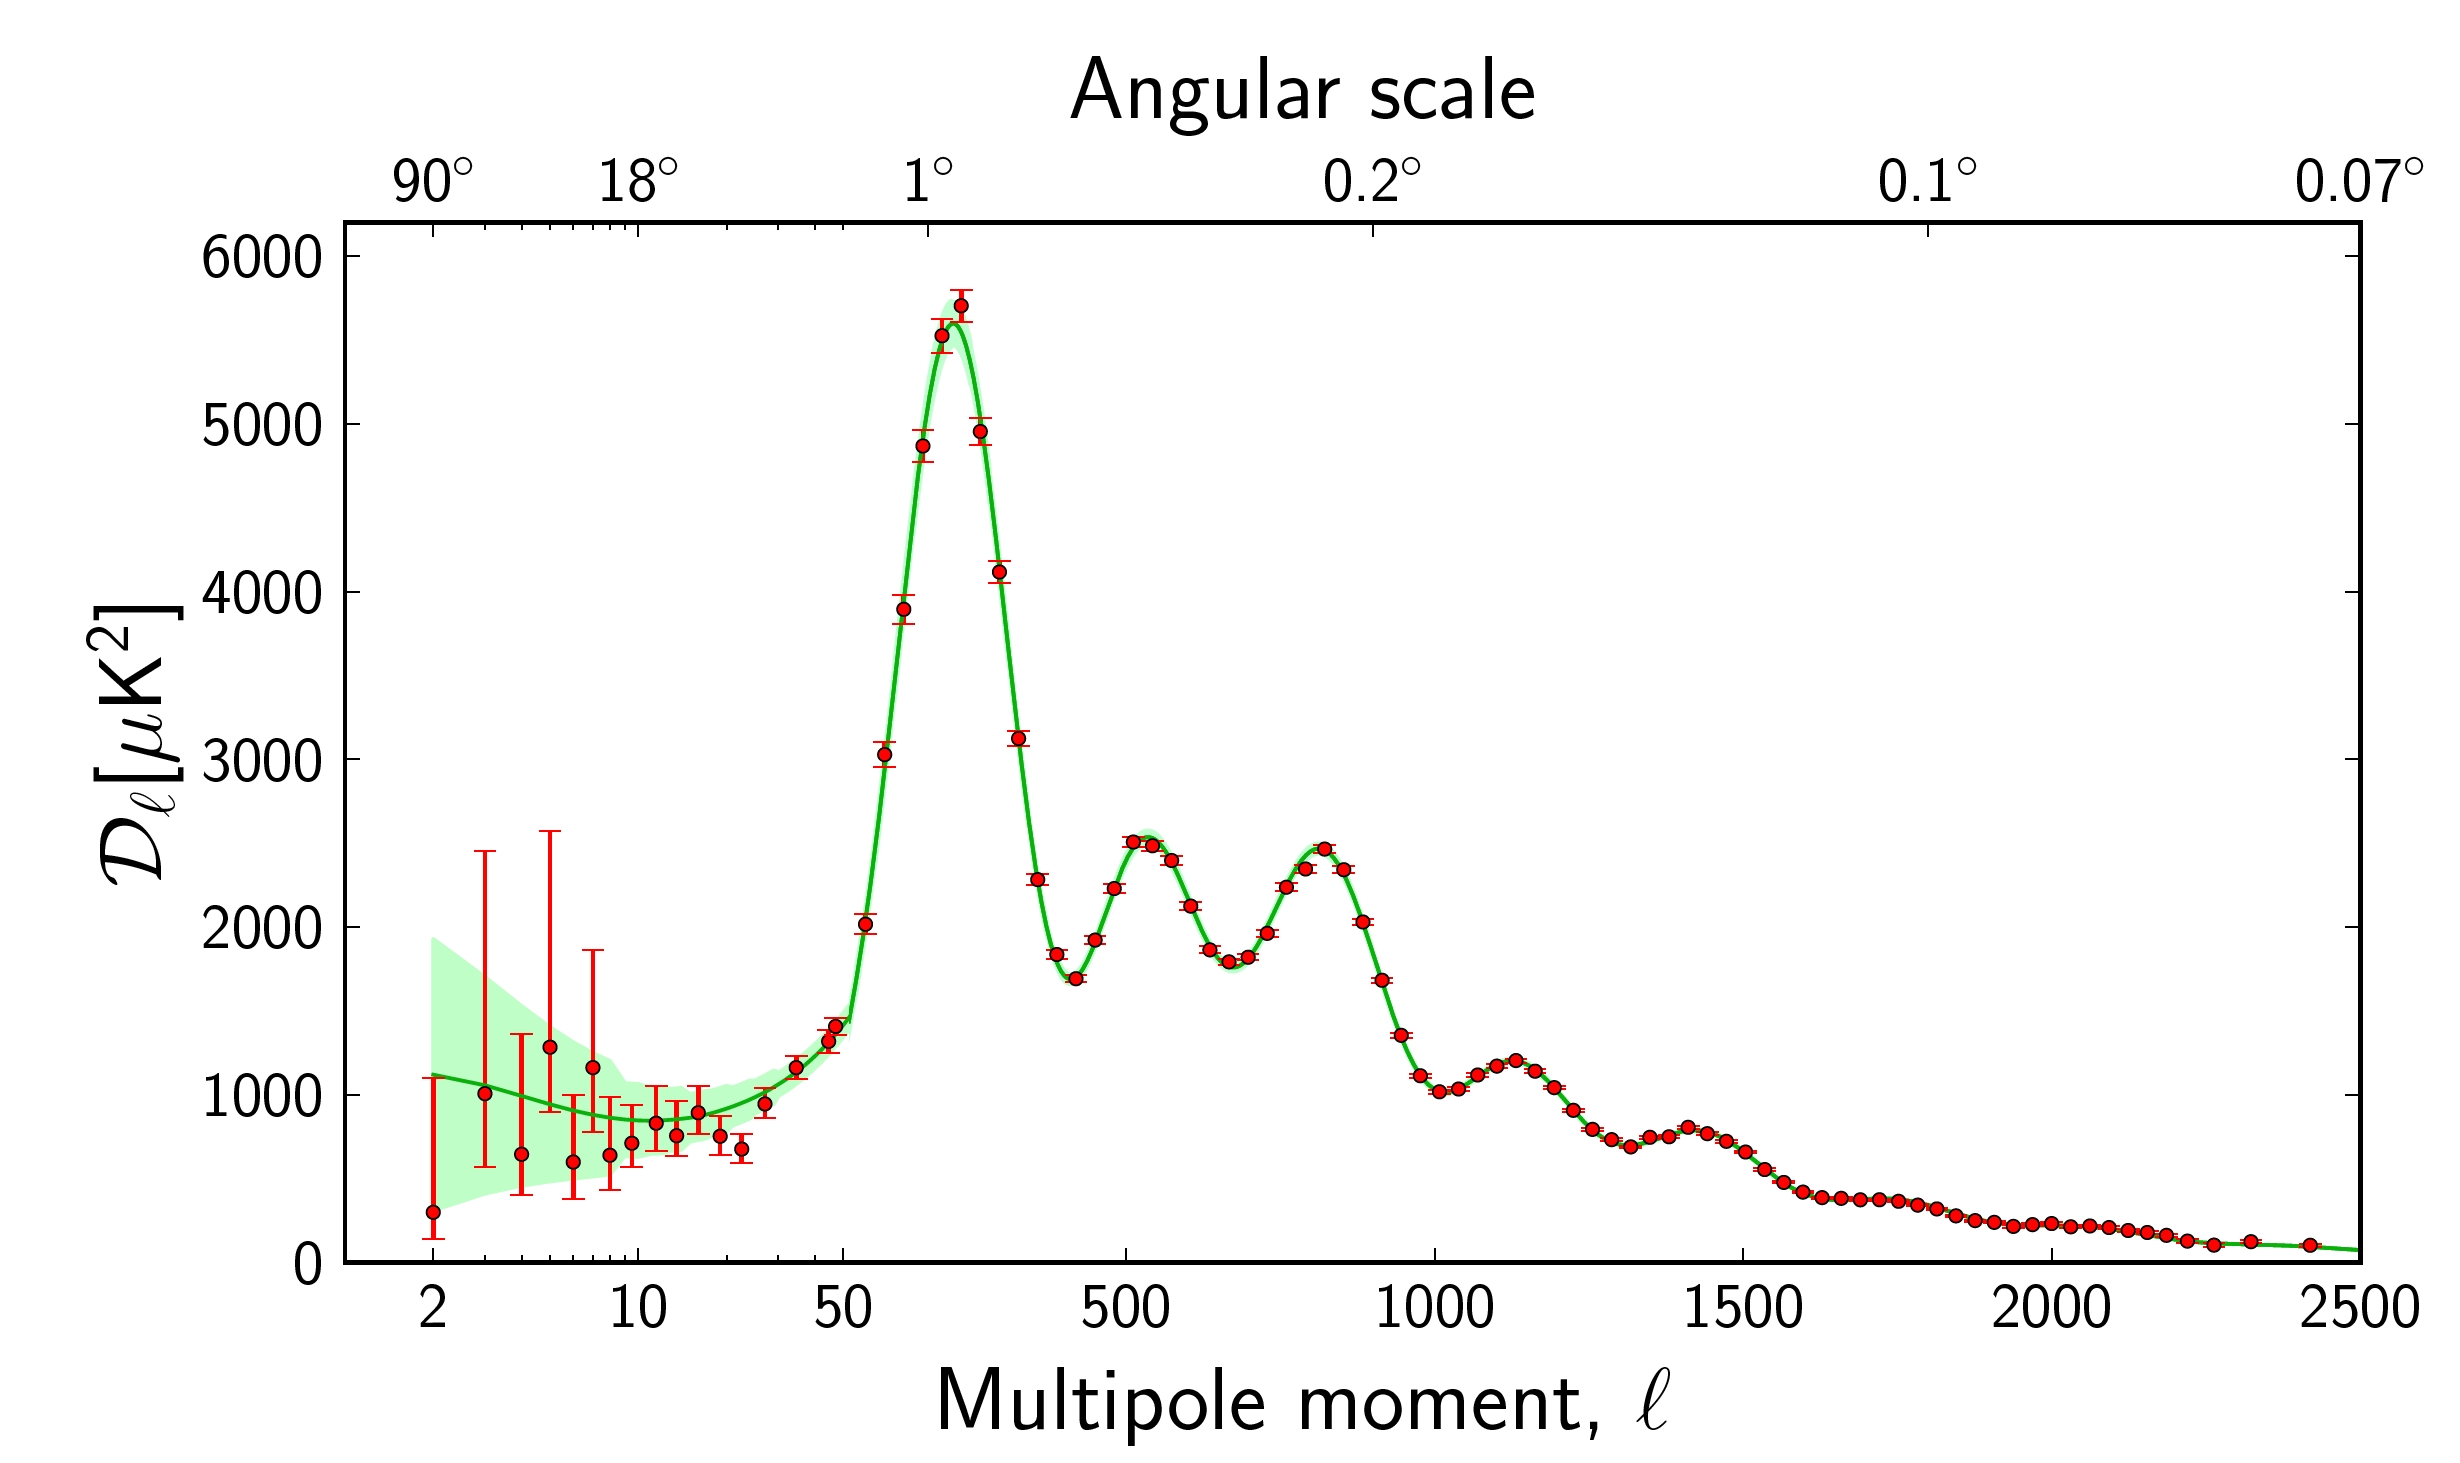
\includegraphics[width=\textwidth]{CMBanisotropies.jpg}
  \caption[CMB anisotropies measured by the Planck experiment]{CMB anisotropies.}
\end{figure}


\begin{table}
  \begin{center}
	\begin{tabular}{cc}
        \hline\hline
        Parameter & 68\% limits \\
        \hline
        $\Omega_\Lambda$ & 0.686 $\pm$ 0.020 \\
        $\Omega_m h^2$ & 0.1423 $\pm$ 0.0029 \\
        $\Omega_b h^2$ & 0.02207 $\pm$ 0.00033 \\
        $\Omega_c h^2$ & 0.1196 $\pm$ 0.0031 \\
        \hline\hline
	\end{tabular}
  \end{center}
  \caption[Cosmological parameters obtained by the Planck Collaboration]{Cosmological parameters obtained by the Planck Collaboration \cite{PlanckXVI:2013}.}
  \label{tab:Planck}
\end{table}

It is determined that dark matter makes up approximately 27\% of the energy density of the universe.